\documentclass{report}
\usepackage[utf8]{inputenc}
\usepackage{listings}
\usepackage{xcolor}
\usepackage{graphicx}
\usepackage{caption} 
\usepackage{helvet}
\renewcommand{\familydefault}{\sfdefault}

\definecolor{codegreen}{rgb}{0,0.6,0}
\definecolor{codegray}{rgb}{0.5,0.5,0.5}
\definecolor{codepurple}{rgb}{0.58,0,0.82}
\definecolor{backcolour}{rgb}{0.95,0.95,0.95}

\lstdefinestyle{mystyle}{
    backgroundcolor=\color{backcolour},   
    commentstyle=\color{codegreen},
    keywordstyle=\color{magenta},
    numberstyle=\tiny\color{codegray},
    stringstyle=\color{codepurple},
    basicstyle=\ttfamily\footnotesize,
    breakatwhitespace=false,         
    breaklines=true,                 
    captionpos=b,                    
    keepspaces=true,                 
    numbers=left,                    
    numbersep=5pt,                  
    showspaces=false,                
    showstringspaces=false,
    showtabs=false,                  
    tabsize=2
}

\lstset{style=mystyle}

\title{PC40 UPC Report}
\author{Esteban Becker}
\date{October 2022}

\begin{document}

\maketitle

\tableofcontents

\chapter{Introduction}

\chapter{Work sharing, synchronization}

\section{Conversion table}

To optimize the code we can parallelize the for loop. To do it correctly we will not use a test in the loop to distribute the work but change the initiation and the step of the for loop.\newline
We have to add a upc\_barrier to be sure all the work is finished before the results are printed.

\begin{lstlisting}[language=C]
#include <stdio.h>
#include <upc.h>
#define TBL_SZ 12

int main(){
    static shared int fahrenheit[TBL_SZ];
    static shared int step=10; 
    int celsius, i;

    //Create the conversion table
    upc_forall(i=MYTHREAD;i<TBL_SZ;i+=THREADS;i){
        celsius=step*i;
        fahrenheit[i]=celsius*(9.0/5.0)+32;
    }
    //Sync all threads
    upc_barrier;

    //Print the conversion table
    if(MYTHREAD==0)

    for(i=0;i<TBL_SZ;i++){
        celsius=step*i;
        printf("%d \t %d \n", fahrenheit[i], celsius);
    }
}

\end{lstlisting}


\chapter{Shared arrays, blocked shared arrays}



\section{Vector addition}

To add two vector vector we can share the work between threads.

\begin{lstlisting}[language=C]
#include<upc_relaxed.h> 
#define N 100 
shared int v1[N], v2[N], v1plusv2[N]; 
void main() 
{ 
    int i; 
    for(i=0;i<N;i++){
        if(MYTHREAD==i%THREADS) 
        v1plusv2[i]=v1[i]+v2[i] ; 
    }
}
\end{lstlisting}

We can change the loop to avoid the code doing a check for each iteration.

\begin{lstlisting}[language=C]
#include<upc_relaxed.h> 
#define N 100 

shared int v1[N], v2[N], v1plusv2[N]; 
void main() 
{ 
    int i; 
    for(i=MYTHREAD; i<N; i+=THREADS){
        v1plusv2[i]=v1[i]+v2[i] ; 
    }
}
\end{lstlisting}

The shared data are distributed in round rubbish fashion. Here the default distribution yields is an efficient implementation in this case

\section{Matrix vector multiplication}

\begin{lstlisting}[language=C]
shared int a[THREADS][THREADS] ; //Matrix A
shared int b[THREADS], c[THREADS] ; //Vector B and C
void main (void) 

{
    int i, j; 
    //Using upc_forall to share the work
    upc_forall( i = 0 ; i < THREADS ; i++; i){
    c[i] = 0;
        for ( j= 0 ; j < THREADS ; j++){
            c[i] += a[i][j]*b[j];
        }
    }
}
\end{lstlisting}

Here the data are not well distributed.

\begin{center}
    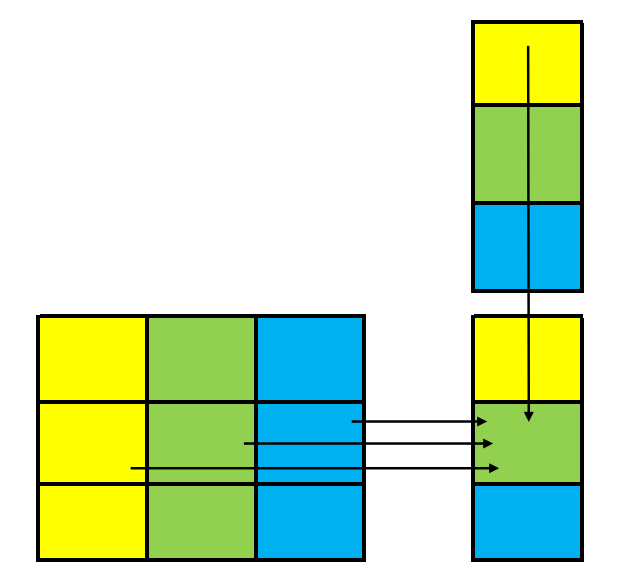
\includegraphics[scale=0.5]{Images/Matrix_vector_unoptimized.png}
    \captionof{figure}{Not optimised data distribution}
    \label{fig1}
\end{center}

To optimise the code we can change the BLOCKSIZE of the matrix a

\begin{lstlisting}[language=C]
// vect_mat_mult.c
#include <upc.h>
shared [THREADS] int a[THREADS][THREADS] ; //Matrix A with a different blocksize
shared int b[THREADS], c[THREADS] ; //Vector B and C
void main (void) 

{
    int i, j; 
    //Using upc_forall to share the work
    upc_forall( i = 0 ; i < THREADS ; i++; i){
    c[i] = 0;
        for ( j= 0 ; j < THREADS ; j++){
            c[i] += a[i][j]*b[j];
        }
    }
}
\end{lstlisting}

\begin{center}
    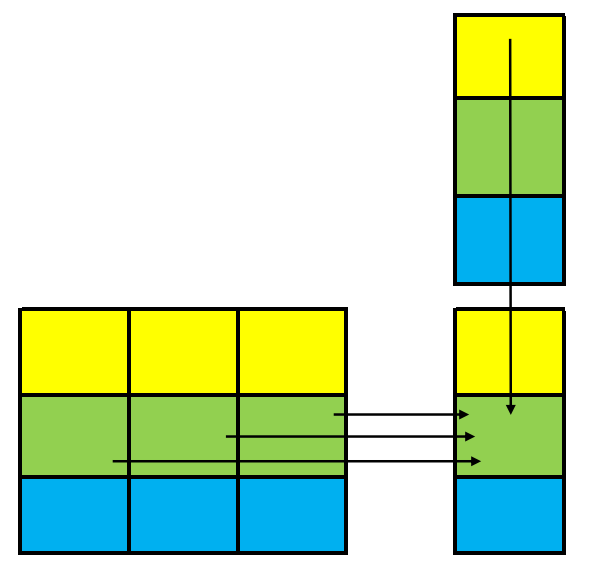
\includegraphics[scale=0.5]{Images/Matrix_vector_optimized.png}
    \captionof{figure}{Optimised data distribution}
    \label{fig2}
\end{center}

\chapter{Simplified 1D Laplace solver}

\section{The 1D solver in UPC}

To implement the 1D in UPC we can to the following code:

\begin{lstlisting}[language=C]
#include <upc_relaxed.h>
#include <stdio.h>
#include <stdlib.h>
#include <time.h>

#define TOTALSIZE 	800

//== declare the x, x_new, b arrays in the shared space with size of TOTALSIZE
shared double x[TOTALSIZE];
shared double x_new[TOTALSIZE];
shared double b[TOTALSIZE];

void init();

int main(int argc, char **argv){
    int j;

    init();
    upc_barrier;

    //== add a for loop which goes through the elements in the x_new array
    for( j=1; j<TOTALSIZE-1; j++ ){
        //== insert an if statement to do the work sharing across the threads
        if( j % THREADS == MYTHREAD){
            x_new[j] = 0.5*( x[j-1] + x[j+1] + b[j] );
        }
    }

    //Print the result with the first thread
    if( MYTHREAD == 0 ){
        printf("   b   |    x   | x_new\n");
        printf("=============================\n");

        for( j=0; j<TOTALSIZE; j++ )
            printf("%1.4f | %1.4f | %1.4f \n", b[j], x[j], x_new[j]);
    }

    return 0;
}

void init(){
    int i;

    if( MYTHREAD == 0 ){
        srand(time(NULL));

        for( i = 0; i<TOTALSIZE; i++ ){
            b[i] = (double)rand() / RAND_MAX;
            x[i] = (double)rand() / RAND_MAX;
        }
    }
}

\end{lstlisting}

This implementation isn't optimise cause each thread will check an IF statement even if it's not there work. To avoid the race condition, we can add two upc\_barrier, one after the initialisation and another before the printing

\begin{center}
    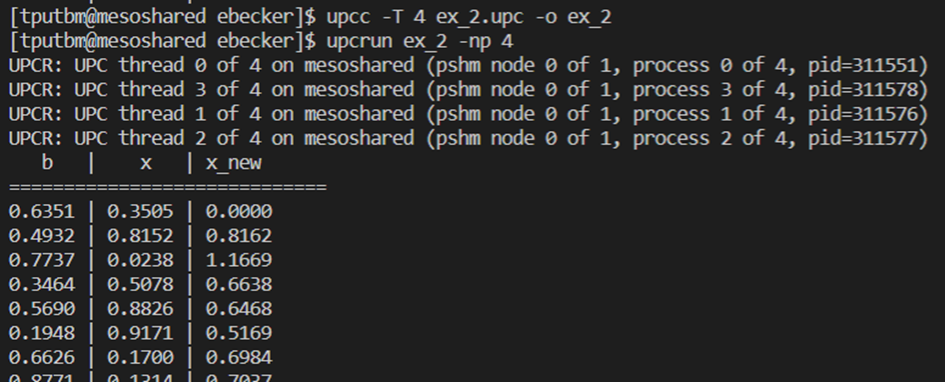
\includegraphics[scale=0.75]{Images/1rst_output.png}
    \captionof{figure}{Output of the 1rst 1D Laplace solver}
    \label{fig3}
\end{center}

\section{Optimize the code}

\subsection{Avoiding the if condition}
To avoid the code to check an if condition we can use the following code:

\begin{lstlisting}[language=C]
    for(int j=MYTHREAD; j<TOTALSIZE-1; j+=THREADS ){
        x_new[j] = 0.5*( x[j-1] + x[j+1] + b[j] );
    }
\end{lstlisting}

\subsection{Blocked arrays}

To optimize the memory distribution we can set a BLOCKSIZE

\begin{lstlisting}[language=C]
#include <upc_relaxed.h>
#include <stdio.h>
#include <stdlib.h>
#include <time.h>

#define BLOCKSIZE 16

//==> declare the x, x_new and b arrays in the shared space with size of 
//    BLOCKSIZE*THREADS and with blocking size of BLOCKSIZE
shared [BLOCKSIZE] double x[BLOCKSIZE*THREADS];
shared [BLOCKSIZE] double x_new[BLOCKSIZE*THREADS];
shared [BLOCKSIZE] double b[BLOCKSIZE*THREADS];

void init();

int main(int argc, char **argv){
    int j;

    init();
    upc_barrier;
    //==> insert a upc_forall statement to do work sharing while 
    //    respecting the affinity of the x_new array
    upc_forall( j=1; j<(BLOCKSIZE*THREADS)-1; j++; &x_new[j] ){
        x_new[j] = 0.5*( x[j-1] + x[j+1] + b[j] );
    }
    upc_barrier;

    if( MYTHREAD == 0 ){
        printf("   b   |    x   | x_new\n");
        printf("=============================\n");

        for( j=0; j<BLOCKSIZE*THREADS; j++ )
            printf("%1.4f | %1.4f | %1.4f \n", b[j], x[j], x_new[j]);
    }

    return 0;
}

void init(){
    int i;

    if( MYTHREAD == 0 ){
        srand(time(NULL));

        for( i=0; i<BLOCKSIZE*THREADS; i++ ){
            b[i] = (double)rand() / RAND_MAX;
            x[i] = (double)rand() / RAND_MAX;
        }
    }
}


\end{lstlisting}

\begin{center}
    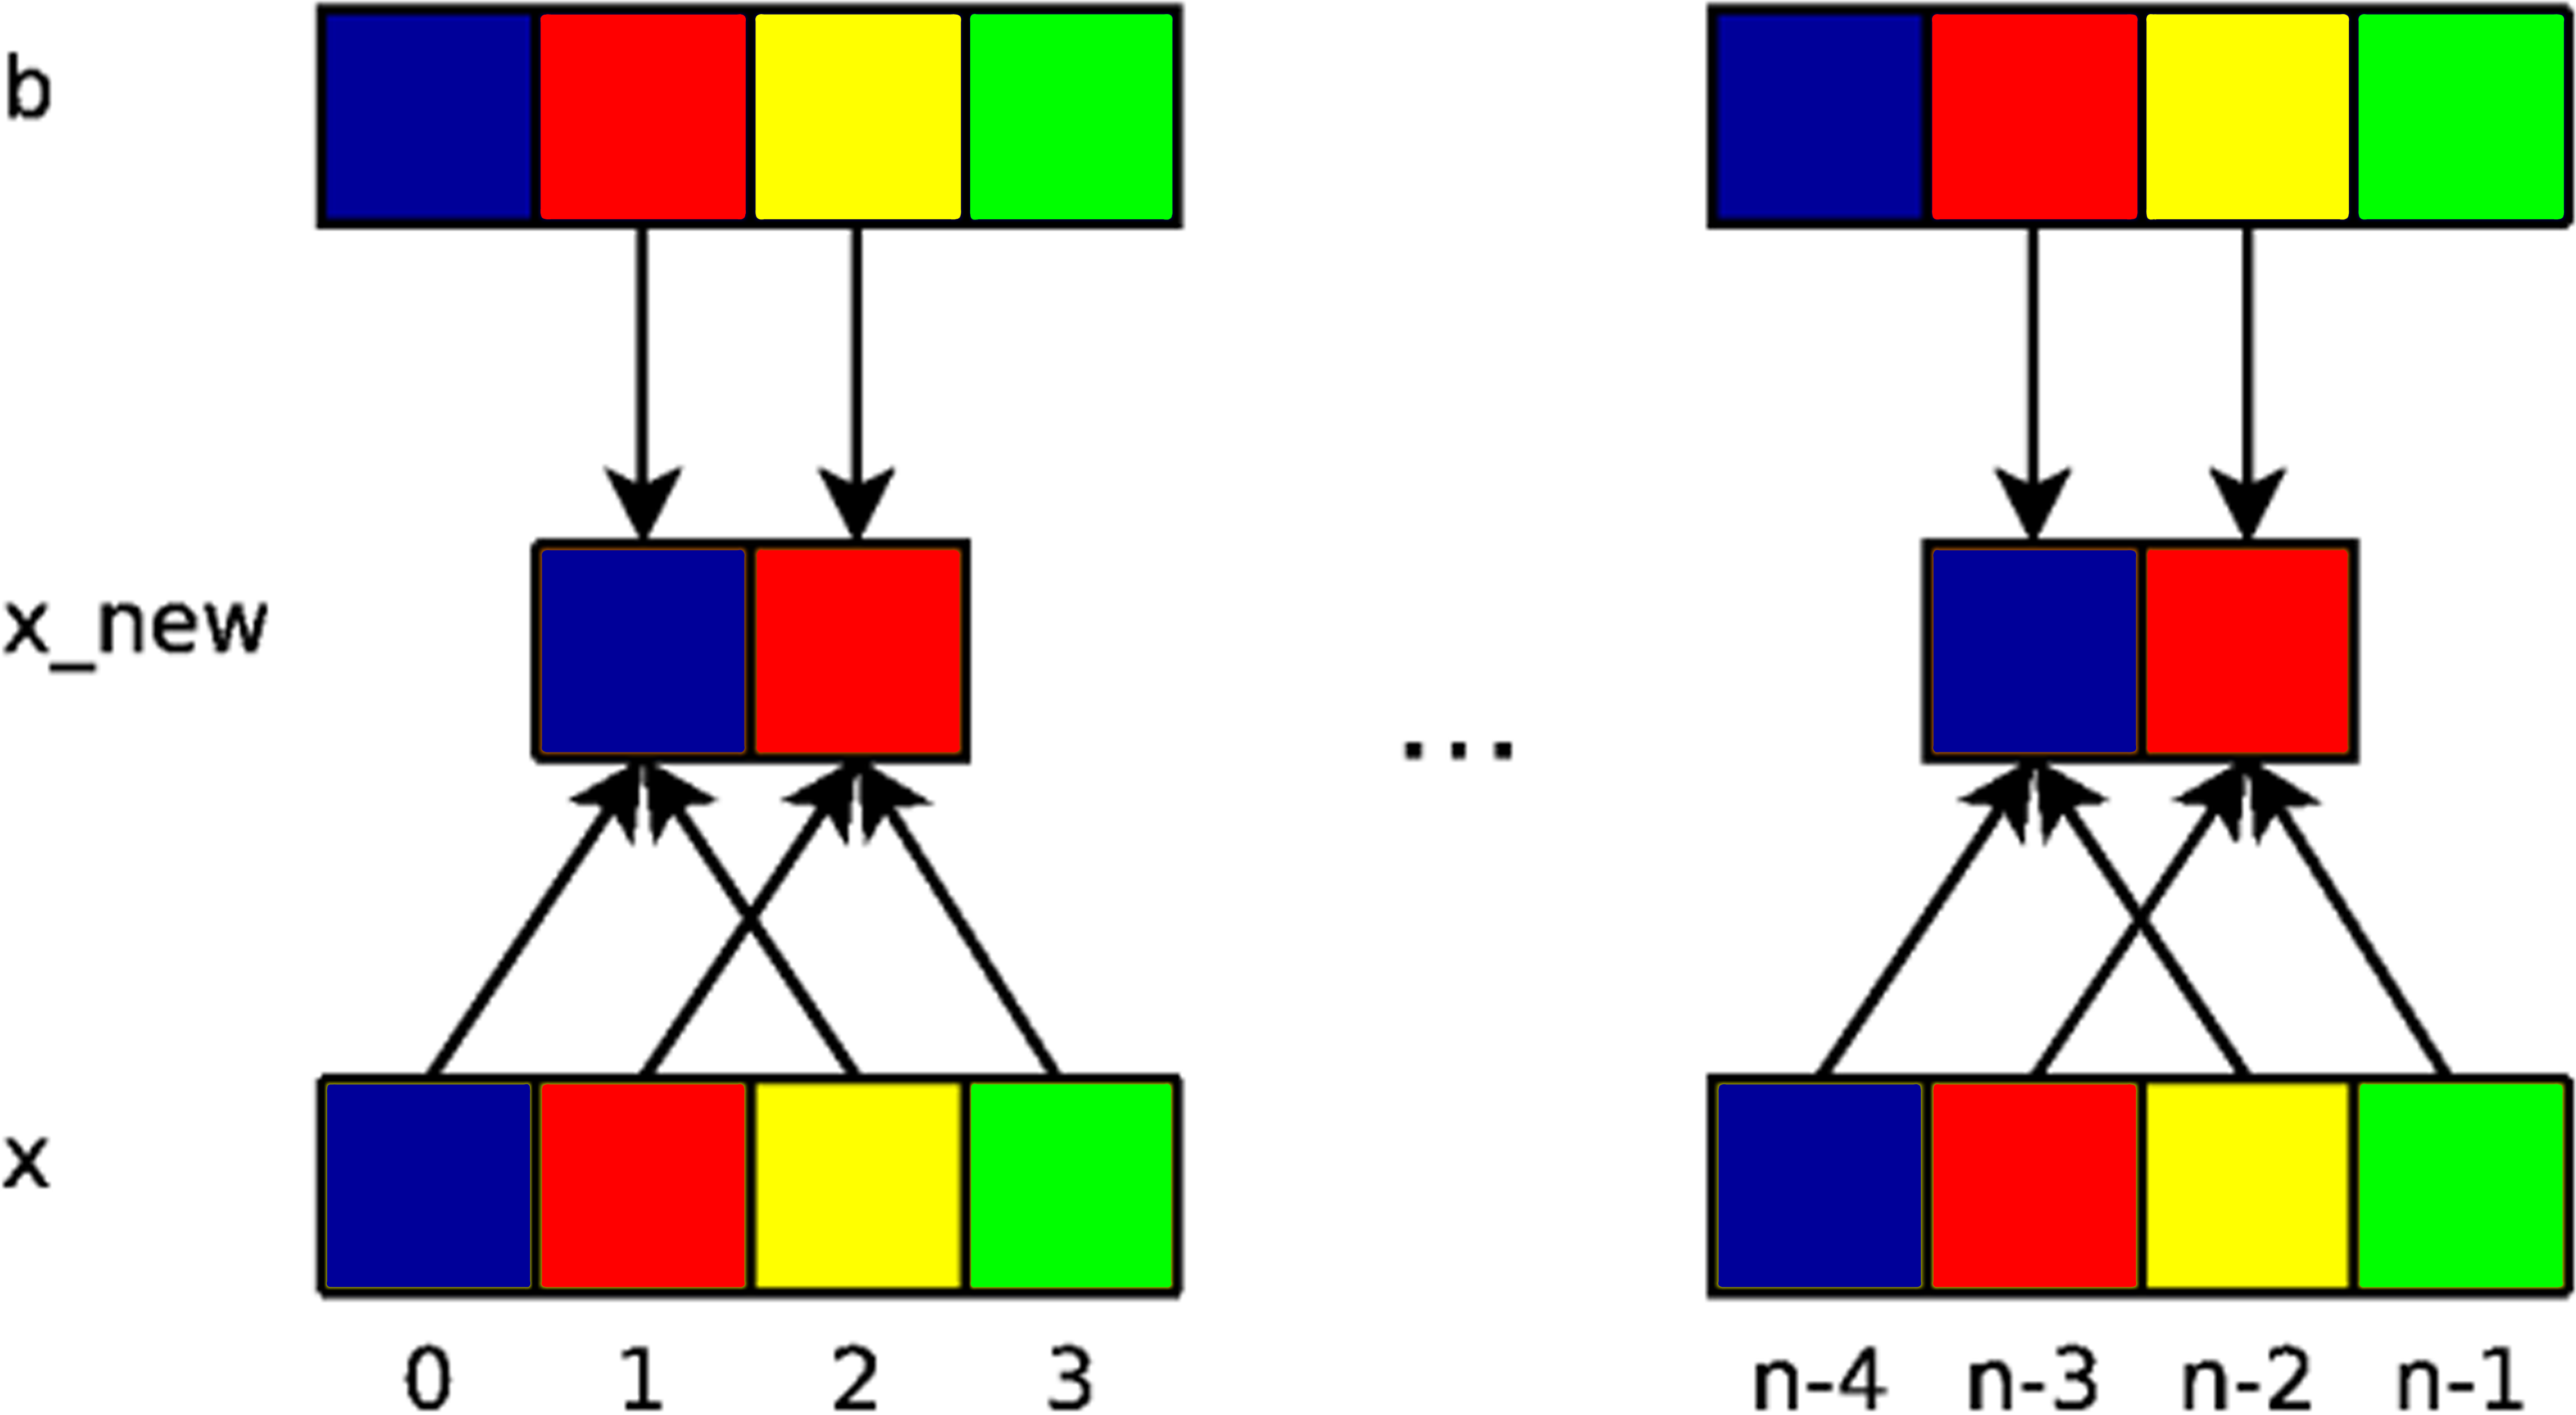
\includegraphics[scale=0.070]{Images/Laplace_unoptimized_da.png}
    \captionof{figure}{Unoptimise data distribution}
    \label{fig4}
    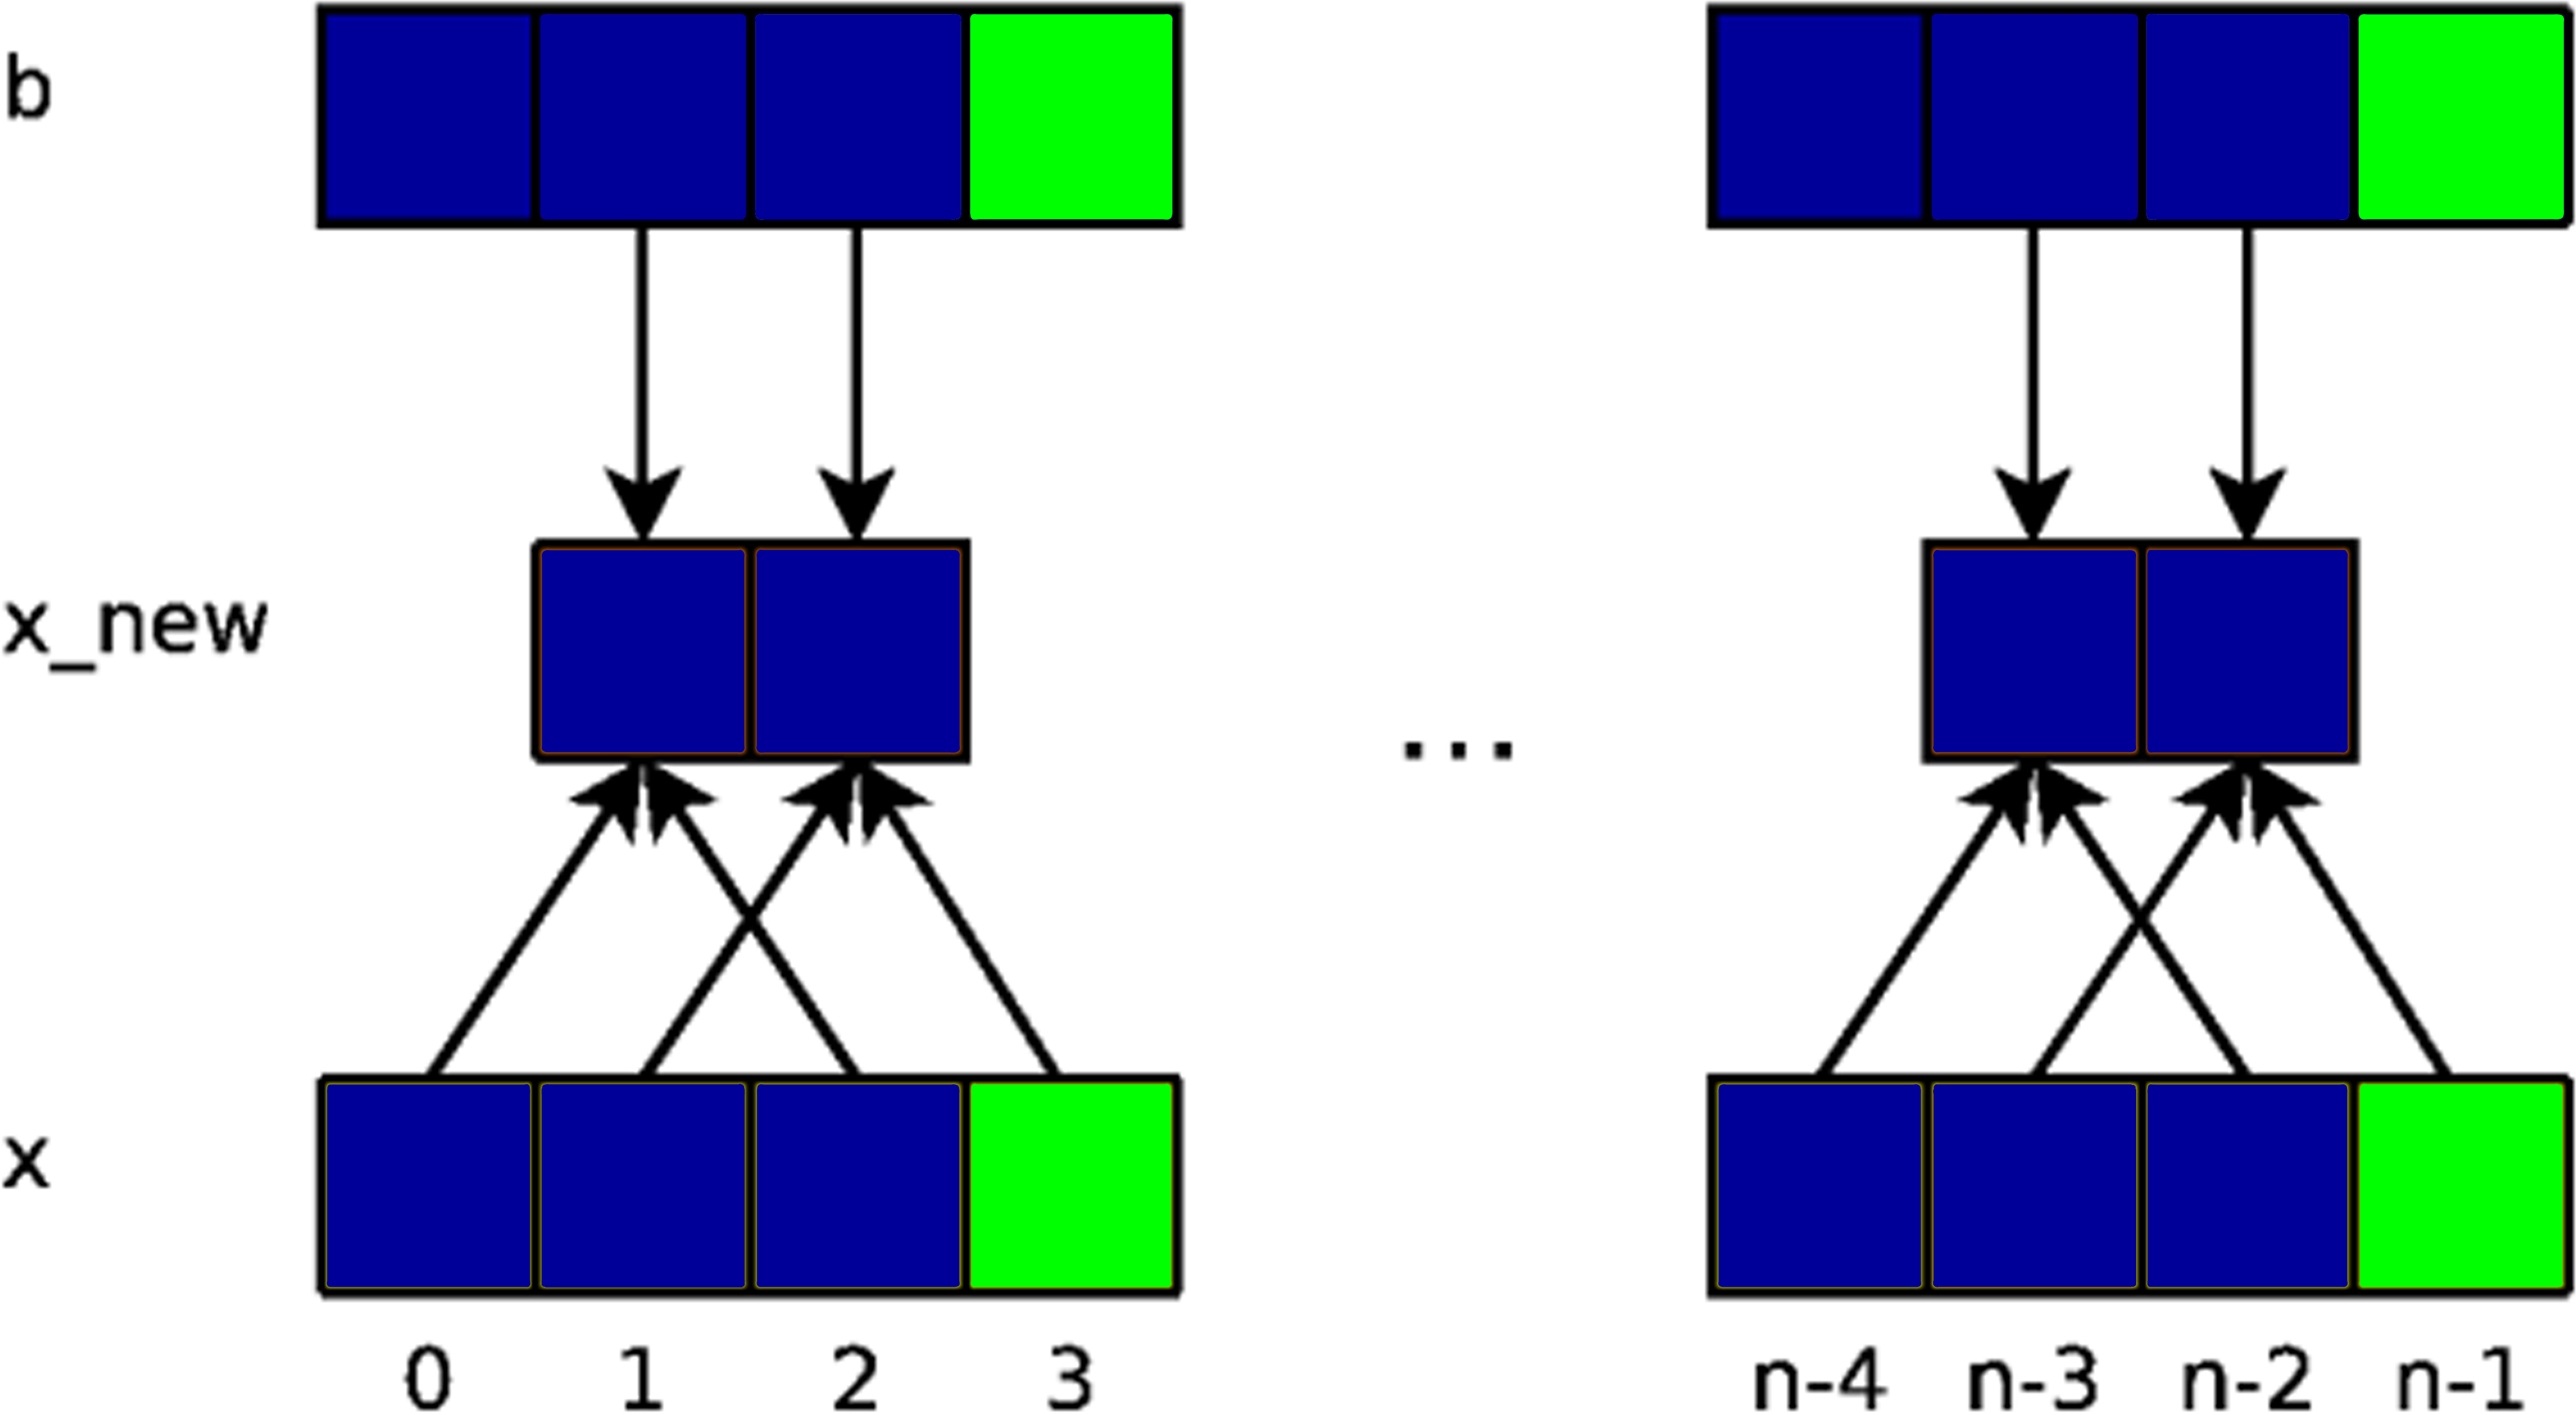
\includegraphics[scale=0.070]{Images/Lapalce_optmized_data.png}
    \captionof{figure}{Optimise data distribution}
    \label{fig5}
\end{center}

With the schema we can see that when the data are grouped together, there is more local shared memory access than the normal distribution.

\section{Synchronization}

\begin{lstlisting}[language=c]
#include <upc_relaxed.h>
#include <stdio.h>
#include <stdlib.h>
#include <time.h>
#define BLOCKSIZE 16

shared [BLOCKSIZE] double x[BLOCKSIZE*THREADS];
shared [BLOCKSIZE] double x_new[BLOCKSIZE*THREADS];
shared [BLOCKSIZE] double b[BLOCKSIZE*THREADS];

void init();

int main(int argc, char **argv){
    int j;
    int iter;

    init();

    // add two barrier statements, to ensure all threads finished computing
    // x_new[] and to ensure that all threads have completed the array
    // swapping.
    for( iter=0; iter<10000; iter++ ){
        upc_forall( j=1; j<BLOCKSIZE*THREADS-1; j++; &x_new[j] ){
            x_new[j] = 0.5*( x[j-1] + x[j+1] + b[j] );
        }

        //UPC barrier needed to ensure all threads have finished computing x_new[]
        upc_barrier;

        upc_forall( j=0; j<BLOCKSIZE*THREADS; j++; &x_new[j] ){
            x[j] = x_new[j];
        }

        //UPC barrier needed to ensure all threads have finished swapping x[] and x_new[]
        upc_barrier;
    }

    if( MYTHREAD == 0 ){
        printf("   b   |    x   | x_new\n");
        printf("=============================\n");

        for( j=0; j<BLOCKSIZE*THREADS; j++ )
            printf("%1.4f | %1.4f | %1.4f \n", b[j], x[j], x_new[j]);
    }

    return 0;
}

void init(){
    int i;

    if( MYTHREAD == 0 ){
        srand(time(NULL));

        for( i=0; i<BLOCKSIZE*THREADS; i++ ){
            b[i] = (double)rand() / RAND_MAX;
            x[i] = (double)rand() / RAND_MAX;
        }
    }
    upc_barrier;
}

\end{lstlisting}

To implement the iteration we have to avoid the race condition by adding two upc\_barrier at the lines 28 and 35

\section{Convergence}
We keep track of the maximum difference between the \textit{x} and \textit{xmax}.
To check if the code reached to convergence we can use a collective operation with the following line:
\begin{lstlisting}[language=c]
upc_all_reduceD( &diffmax, diff, UPC_MAX,THREADS,1,NULL,UPC_OUT_ALLSYNC);
\end{lstlisting}

To finally obtain this code:

\begin{lstlisting}[language=c]
#include <upc.h>
#include <upc_collective.h> 
#include <stdio.h>
#include <math.h>

#define TOTALSIZE 100
#define EPSILON 0.000001

shared [TOTALSIZE] double x[TOTALSIZE*THREADS];
shared [TOTALSIZE] double x_new[TOTALSIZE*THREADS];
shared [TOTALSIZE] double b[TOTALSIZE*THREADS];
shared double diff[THREADS];
shared double diffmax;

void init(){
    int i;

    for( i = 0; i < TOTALSIZE*THREADS; i++ ){
        b[i] = 0;
        x[i] = 0;
    }

    b[1] = 1.0;
    b[TOTALSIZE*THREADS-2] = 1.0;
}

int main(){
    int j;
    int iter = 0;

    if( MYTHREAD == 0 )
        init();

    upc_barrier;

    while( 1 ){
        iter++;
        diff[MYTHREAD] = 0.0;

        upc_forall( j=1; j<TOTALSIZE*THREADS-1; j++; &x_new[j] ){
            x_new[j] = 0.5 * ( x[j-1] + x[j+1] + b[j] );

            if( diff[MYTHREAD] < x_new[j] - x[j] )
                diff[MYTHREAD] = x_new[j] - x[j];
        }

        // Each thread as a local value for diff
        // The maximum of those values should be used to check
        // the convergence.

        upc_all_reduceD( &diffmax, diff, UPC_MAX,THREADS,1,NULL,UPC_OUT_ALLSYNC);

        printf("diff max = %f \n", diffmax);

        if( diffmax <= EPSILON )
            break;
        if( iter > 10000 )
            break;

        upc_forall( j=0; j<TOTALSIZE*THREADS; j++; &x_new[j] ){
            x[j] = x_new[j];
        }
        upc_barrier;
    }

    
    if( MYTHREAD == 0 ){
        for(j=0; j<TOTALSIZE*THREADS; j++){
            printf("%f\t", x_new[j]);
        }
        printf("\n");
    }

    return 0;
}
\end{lstlisting}

\chapter{2D Heat conduction}

\section{First UPC program}

To create the first UPC version we spread the work between all the threads and optimize the data blocksize

\begin{lstlisting}[language=c]
#include <stdio.h>
#include <math.h>
#include <sys/time.h>
#include <upc_relaxed.h>
#include <upc_collective.h> 

#define N 30

shared [(N+2)*(N+2)/THREADS] double grid[N+2][N+2], new_grid[N+2][N+2];
shared double dTmax[THREADS];
shared double diffmax;

void initialize(void)
{
    int j;

    /* Heat one side of the solid */
    upc_forall( j=1; j<N+1; j++; j)
    {
        grid[0][j] = 1.0;
        new_grid[0][j] = 1.0;
    }
    upc_barrier;
}

int main(void)
{
    struct timeval ts_st, ts_end;
    double dT, epsilon, time;
    int finished, i, j, k, l;
    double T;
    int nr_iter;

    initialize();

    /* Set the precision wanted */
    epsilon  = 0.0001;
    finished = 0;
    nr_iter = 0;

    /* and start the timed section */
    gettimeofday( &ts_st, NULL );

    do
    {
        dTmax[MYTHREAD] = 0.0; 
        upc_forall( i=1; i<N+1; i++; i*THREADS/(N+2))
        {
            //Do the new grid calculation
            for( j=1; j<N+1; j++ )
            {
                T = 0.25 *
                    (grid[i+1][j] + grid[i-1][j] +
                     grid[i][j-1] + grid[i][j+1]); /* stencil */
                dT = T - grid[i][j]; /* local variation */
                new_grid[i][j] = T;
                if( dTmax[MYTHREAD] < fabs(dT) )
                    dTmax[MYTHREAD] = fabs(dT); /* max variation in this iteration */
            }
        }
        upc_barrier;
        upc_all_reduceD( &diffmax, dTmax, UPC_MAX,THREADS,1,NULL,UPC_OUT_ALLSYNC);
        if( diffmax < epsilon ) /* is the precision reached good enough ? */
            finished = 1;
        else
        {
            upc_forall( k=0; k<N+2; k++; k)      /* swap the grids */
                for( l=0; l<N+2; l++ )    
                    grid[k][l] = new_grid[k][l]; 
        }
        upc_barrier;
        nr_iter++;
    } while( finished == 0 );

    if(MYTHREAD == 0)
    {
        gettimeofday( &ts_end, NULL ); /* end the timed section */

        /* compute the execution time */
        time = ts_end.tv_sec + (ts_end.tv_usec / 1000000.0);
        time -= ts_st.tv_sec + (ts_st.tv_usec / 1000000.0);

        printf("%d iterations in %.3lf sec\n", nr_iter, time);
    }

    return 0;
}
\end{lstlisting}

\listoffigures
\end{document}
